\documentclass{standalone}

\usepackage{standalone}
\usepackage{tikz}
\usetikzlibrary{er,positioning, calc}

\begin{document}

	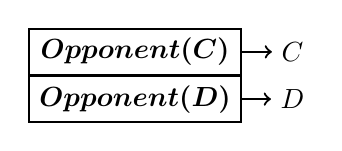
\begin{tikzpicture}
    	\tikzstyle{state}=[minimum width=2.7cm, font=\boldmath];

   	\node[rectangle, draw=black, thick] (0) at (0, 0) [state] {$Opponent(C)$};
    \node (1) at (2, 0) {$C$};
    \draw (0) edge[out=0, in=180, ->, thick] node {} (1);

    \node[rectangle, draw=black, thick] (3) at (0, -0.6) [state] {$Opponent(D)$};
    \node (4) at (2, -.6) {$D$};
    \draw (3) edge[out=0, in=180, ->, thick] node {} (4);
 
	\end{tikzpicture}
\end{document}